\documentclass{standalone}
\usepackage{tikz}

\begin{document}

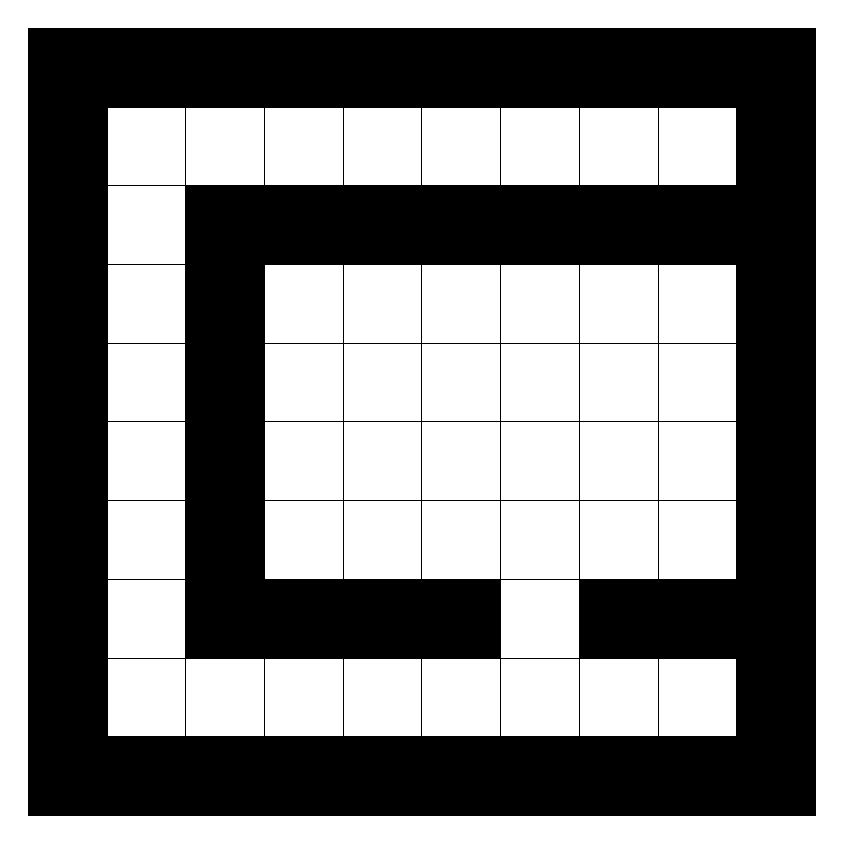
\begin{tikzpicture}
  \draw (0,0) grid (10,10);

  \foreach \x in {0,...,9} {
    \fill (\x,0) rectangle ++(1,1);
    \fill (\x,9) rectangle ++(1,1);
  }
  \foreach \y in {1,...,8} {
    \fill (0,\y) rectangle ++(1,1);
    \fill (9,\y) rectangle ++(1,1);
  }
  \foreach \x/\y in {2/2,2/3,2/4,2/5,2/6,2/7,3/2,4/2,5/2,7/2,8/2,3/7,4/7,5/7,6/7,7/7,8/7} {
    \fill (\x,\y) rectangle ++(1,1);
  }
\end{tikzpicture}

\end{document}